\documentclass[12pt, openany]{report}
\usepackage[utf8]{inputenc}
\usepackage[T1]{fontenc}
\usepackage{amsmath,amsfonts,amssymb}
\usepackage{amssymb}
\usepackage{multicol}
\usepackage[a4paper,left=2.5cm,right=2.5cm,top=2.5cm,bottom=2.5cm]{geometry}
\usepackage[english]{babel}
\usepackage{libertine}
\usepackage{graphicx}
\usepackage{wrapfig}
\usepackage{algorithm}
\usepackage{algpseudocode}
\usepackage{float}
\usepackage{enumitem}
\usepackage{pythonhighlight}
\usepackage[]{titletoc}
\usepackage{empheq}
\usepackage{titlesec}
\usepackage{mathpazo}
\usepackage{xfrac}
\usepackage{textcomp}
\usepackage{mathtools}
\usepackage{caption}
\usepackage{tabularray}
\usepackage{subcaption}
\usepackage[bottom]{footmisc}
\usepackage{pdfpages}
\usepackage{tabularx}
\usepackage{amsthm}
\usepackage[skins]{tcolorbox}
\titleformat{\chapter}[display]
  {\normalfont\bfseries}{}{0pt}{\Huge}
\usepackage{hyperref}
\newcommand{\hsp}{\hspace{20pt}}
\newcommand{\HRule}{\rule{\linewidth}{0.5mm}}
\newcommand{\R}{\mathbb{R}}
\newcommand{\C}{\mathbb{C}}
\theoremstyle{definition}
\newtheorem{thm}{Theorem}[chapter]
\newtheorem{definition}[thm]{Definition}
\newtheorem{lem}[thm]{Lemma}

\hbadness=100000
\begin{document}
\begin{titlepage}
    \begin{sffamily}
    \begin{center}
        
\includegraphics[scale=0.25]{img/page_de_garde.png} \\[1cm]
        \HRule \\[0.4cm]
        { \huge \bfseries LINMA2171 Numerical Analysis \\[0.4cm] }
    
        \HRule \\[1.5cm]
        \textsc{\LARGE Simon Desmidt}\\[1cm]
        \vfill
        \vspace{2cm}
        {\large Academic year 2024-2025 - Q1}
        \vspace{0.4cm}
         
        
\includegraphics[width=0.15\textwidth]{img/epl.png}
        
        UCLouvain\\
    
    \end{center}
    \end{sffamily}
\end{titlepage}

\setcounter{tocdepth}{1}
\tableofcontents
\chapter{Polynomial interpolation}
\(\mathcal{P}_n\) is the set of all real polynomials of degree at most \(n\). 
\begin{itemize}
    \item The Runge phenomenon is the explosion of the polynomial near the boundary of the domain when the interpolation points are chosen to be equidistant. A solution to that is to put more points near the boundary and less in the middle of the domain, e.g. Chebyshev points.
\end{itemize}
\section{Lagrange interpolation}
Let \(x_0,\dots,x_n\) be distinct real numbers. The Lagrange polynomial \(L_k\) of degree \(n\) is such that it is equal to 0 for all \(x_i\), \(i\neq k\) and \(1\) for \(x_k\). This serves as a base for the next interpolations. The general formula for the Lagrange polynomial is 
\begin{equation}
    L_k(x) = \prod_{\substack{i=0\\ i\neq k}}^n \frac{x-x_i}{x_k-x_i}\qquad k=0,1,\dots,n
\end{equation}
\begin{itemize}
    \item Note: we usually denote \(L_k(x;x_0,\dots,x_n)\) or let \(\chi = (x_0,\dots,x_n)\) and \(L_k(x;\chi)\). 
\end{itemize}
\begin{thm}
    Assume that $n\ge 0$. Let $x_i,\: i=0,\dots,n$ be distinct real number and suppose that $y_i,\: i=0,\dots,n$ are real numbers. Then, there is a unique polynomial $p_n\in \mathcal{P}_n$ such that $p_n(x_i)=y_i$ for all $i=0,\dots,n$.
\end{thm}
\begin{definition}
    The polynomial $p_n$ defined by 
    \begin{equation}\label{eq:lagrange}
        p_n(x) = \sum_{k=0}^n y_kL_k(x)
    \end{equation}
    with $L_k$ the Lagrange polynomial ($L_0(x) \equiv 1$), is the Lagrange interpolation polynomial of degree $n$ for the points $(x_i,y_i),\: i=0,\dots,n$.
\end{definition}
\begin{thm}
    Let $f:\R\mapsto \R$, $f\in \mathcal{C}^{n+1}[a,b]$. Then, given that $x\in[a,b]$, there exists $\xi=\xi(x)$ on $(a,b)$ such that 
    \begin{equation}
        f(x)-p_n(x) = \frac{f^{(n+1)}(\xi)}{(n+1)!}\pi_{n+1}(x)
    \end{equation}
    where $\pi_{n+1} = \prod_{i=0}^n(x-x_i)$. Moreover, 
    \begin{equation}
        |f(x)-p_n(x)| \le \frac{M_{n+1}}{(n+1)!}|\pi_{n+1}(x)| \qquad M_{n+1} = \max_{\zeta \in [a,b]}|f^{(n+1)}(\zeta)|
    \end{equation}
\end{thm}
\section{Hermite interpolation}
Let \(x_0,\dots,x_n\) be distinct real numbers. Then, given two sets of real numbers \((y_0,\dots y_n)\) and \((z_0,\dots,z_n)\), there is a unique polynomial \(p_{2n+1}\in \mathcal{P}_{2n+1}\) such that 
\begin{equation}
    p_{2n+1} (x_i) = y_i \qquad p_{2n+1}'(x_i) =z_i \qquad i=0,\dots,n
\end{equation}
The polynomial \(p_{2n+1}\) is called the Hermite interpolation polynomial of degree at most \(2n+1\) for the data points \((x_0,y_0,z_0),\dots,(x_n,y_n,z_n)\). The expression is 
\begin{equation}
    p_{2n+1}(x) = \sum_{k=0}^n \left(H_k(x)y_k + K_k(x)z_k\right) \qquad \begin{cases}
        H_k(x) = (L_k(x))^2(1-2L'_k(x_k)(x-x_k))\\
        K_k(x) = (L_k(x))^2(x-x_k)
    \end{cases}
\end{equation}
where \(L_k(x)\) is the Lagrange polynomial.
\begin{itemize}
    \item The \(H_k(x)\) are such that their derivative is zero for all \(x_i\), and their value is zero for all \(x_i\) except \(x_k\), where it is 1.\[H_k(x_i) = \delta_{ik}\qquad H_k'(x_i) = 0 \qquad \forall i\]
    \item The \(K_k(x)\) are such that their derivative is zero for all \(x_i\) except \(x_k\) where it is one, and their value is zero for all \(x_i\).\[K_k(x_i) = 0\qquad K_k'(x_i) = \delta_{ik} \qquad \forall i\]
    \item [$\rightarrow$] Note: for $n=0$, we define $H_0(x)\equiv 1$ and $K_0(x)\equiv x-x_0$.
\end{itemize}
\section{Neville's algorithm}
Let us assume we are given a set of support points \((x_i,y_i)\), \(i=0,1,\dots,n\), and \(p_n\) is their Lagrange interpolation polynomial. Let us now define the notation \(P_{i_0i_1\dots i_k}\in \mathcal{P}_k\), the polynomial for which \(P_{i_0i_1\dots i_k}(x_{i_j})=y_{i_j}\)  for all \(j=0,1,\dots,k\). We work by recursion, with the following formula:
\begin{equation}
    \begin{cases}
        P_i(x) = y_i\\
        P_{i_0i_1\dots i_k} = \frac{(x-x_{i_0})P_{i_1i_2\dots i_k}(x) - (x-x_{i_k})P_{i_0i_1\dots i_{k-1}}(x)}{x_{i_k}-x_{i_0}}
    \end{cases}
\end{equation}
Example:\\
Let us have four points \((x_0,y_0),\dots(x_3,y_3)\). We want the polynomial interpolating all of them, using Neville's algorithm. 
\begin{figure}[H]
    \centering
    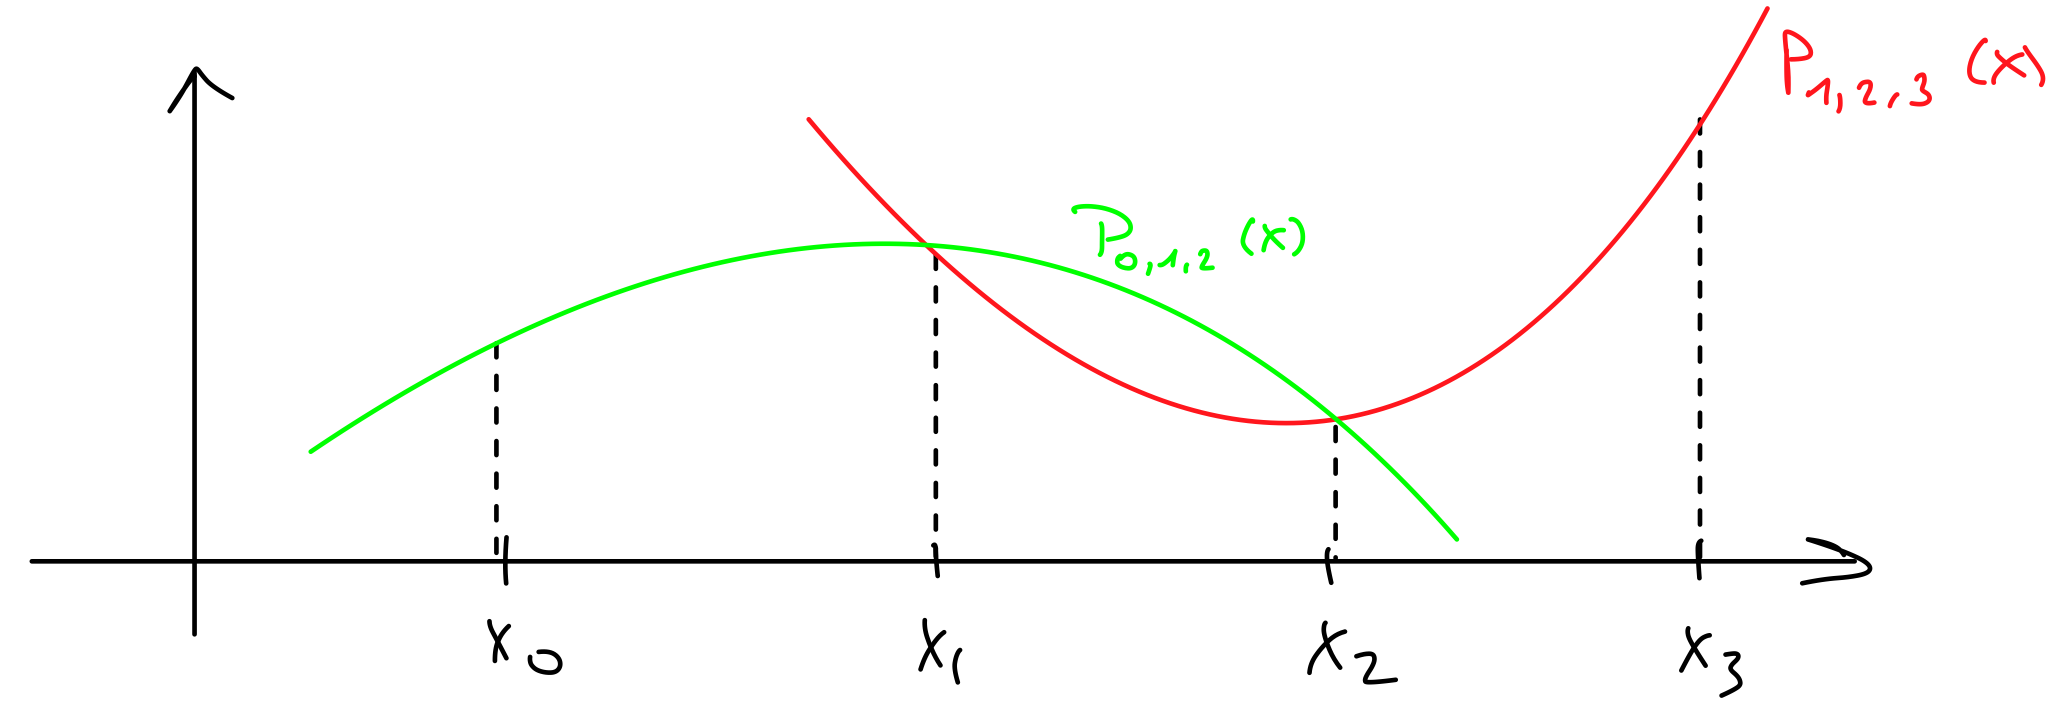
\includegraphics[width=0.5\linewidth]{img/neville.png}
\end{figure}
Here, 
\begin{equation}
    P_{0123}(x) = \frac{x-x_0}{x_3-x_0}\color{red}P_{123}(x)\color{black}+\frac{x_3-x}{x_3-x_0}\color{green}P_{012}(x)\color{black}
\end{equation}
\section{Newton's interpolation formula}
Newton's interpolation formula is used to evaluate polynomials with a computer, as it only needs to compute each operation \((x-x_i)\) one time. We write it like:
\begin{equation}
    p_n(x) = \left(\left(\dots\left(y_{0\dots n}(x-x_n)+y_{0\dots n-1}\right)(x-x_{n-1})+y_{0\dots n-2}\right)(x-x_{n-2})+\dots\right) + y_0
\end{equation}
And the recursive formula is
\begin{equation}
    P_{i_0i_1\dots i_k}= P_{i_0i_1\dots i_{k-1}}(x) + y_{i_0i_1\dots i_k}(x-x_{i_0})(x-x_{i_1})\dots(x-x_{i_{k-1}})
\end{equation}
\section{Linear algebra approach}
Let \((\phi_0,\dots,\phi_n)\) be a basis of \(\mathcal{P}_n\), which is known to be an \((n+1)\)-dimensional linear space. The interpolation polynomial can thus be expressed in a unique way in the basis:
\begin{equation}
    p_n(x) = \sum_{i=0}^n a_i\phi_i(x)
\end{equation}
and the coefficient are obtained by solving the linear system
\begin{equation}
    \begin{bmatrix}
        \phi_0(x_0) & \phi_1(x_0) & \dots & \phi_n(x_0)\\
        \phi_0(x_1) & \phi_1(x_1) & \dots & \phi_n(x_1)\\
        \vdots  & \vdots & \ddots & \vdots\\
        \phi_0(x_n) & \phi_1(x_n) & \dots & \phi_n(x_n)\\
    \end{bmatrix}\begin{bmatrix}
        a_0\\ a_1\\ \vdots \\a_n\\
    \end{bmatrix} = \begin{bmatrix}
        y_0 \\y_1\\\vdots \\ y_n\\
    \end{bmatrix}
\end{equation}
This is called a Vandermonde matrix, and its determinant is 
\begin{equation}
    \det(V) = \prod_{0\le i< j\le n}(x_j-x_i)
\end{equation}
which is always non zero, as the \(x_i\) are disinct, and the system has one unique solution. 
\begin{itemize}
    \item [\(\rightarrow\)] Note: the condition number\footnote{It is a measure of the reaction of the system to a small perturbation} of such a matrix grows exponentially with \(n\). 
\end{itemize}
\section{Barycentric interpolation formula}
This formula is interesting, because it is numerically stable, contrary to the linear algebra method described before. We use the following notation, called the nodal polynomial:
\begin{equation}
    \pi_{n+1}(x) = \prod_{i=0}^n (x-x_i)
\end{equation}
We now define 
\begin{equation}
    \lambda_j = \frac{1}{\prod_{k\neq j}(x_j-x_k)}
\end{equation}
The modified Lagrange formula is then 
\begin{equation}\label{eq:barycentric1}
    p_n(x) = \pi_{n+1}(x) \sum_{j=0}^n \frac{\lambda_j}{x-x_j}y_i
\end{equation}
For the polynomial \(p_n(x) = 1\), we have the following expression:\[1 = \pi_{n+1}(x) \sum_{j=0}^n \frac{\lambda_j}{x-x_j}\] and thus we generally prefer to use the equivalent formula for equation \eqref{eq:barycentric1}:
\begin{equation}\label{eq:barycentric2}
    p_n(x) = \sum_{j=0}^n \frac{\lambda_jy_j}{x-x_j} / \sum_{j=0}^n \frac{\lambda_j}{x-x_j}
\end{equation}
for all \(x\notin \{x_0,\dots,x_n\}\).
\section{Trigonometric interpolation}
Let us consider the evenly spaced points \(x_j = \frac{2\pi j}{N}\), \(j=0,\dots,N\), on the interval \([0,2\pi]\), and the interpolation values \(f_0,\dots, f_N\in \mathbb{C}\), with \(f_0=f_N\). The trigonometric interpolation problem consists of finding \(\beta_k\) such that 
\begin{equation}
    p(x) = \sum_{k=0}^{N-1}\beta_ke^{ikx}\text{ such that } p(x_j) = f_j\qquad j=0,\dots,N-1
\end{equation}
\begin{itemize}
    \item [\(\rightarrow\)] Note: the bound is \(N-1\) because the last condition \(p(x_N) = f_N\) is satisfied when the others are (periodicity). 
\end{itemize}
This is equivalent to the generalization to \(\mathbb{C}\) of the polynomial interpolation problem: if we denote \(\omega \coloneqq e^{ix}\), the complex polynomial is 
\begin{equation}
    P(\omega) = \sum_{k=0}^{N-1} \beta_k \omega^k
\end{equation}
The Vandermonde matrix in the complex case is defined as in the real case. We denote it \(W\). \\
Theorem: \(W^*W=NI\) for a complex Vandermonde matrix in an interpolation problem. \\

From this, the solution to the interpolation problem is solved by multiplying both sides by \(W^*\). We get 
\begin{equation}
    \beta = \frac{1}{N}W^*f \Longrightarrow \beta_k = \frac{1}{N}\sum_{j=0}^{N-1}f_j e^{-i2\pi kj/N} \qquad k=0,\dots,N-1
\end{equation}
And that is the discrete Fourier transform (DFT)
\section{Rational interpolation}
Let the interpolation points be \(x_0< x_1<\dots<x_\sigma\), with the values \(y_0,\dots,y_\sigma\in\R\). We define the polynomial
\begin{align}\label{eq:rational}
    \Phi(x) &= \frac{p_\mu(x)}{q_\nu(x)} \qquad p_\mu \in\mathcal{P}_\mu, q_\nu\in \mathcal{P}_\nu\\
    &\text{such that } \Phi(x_i)=y_i\qquad i = 0,\dots,\sigma
\end{align}
The interpolation polynomial can be written 
\begin{equation}
    \Phi(x) = \frac{\sum_{k=0}^\mu a_kx^k}{\sum_{k=0}^\nu b_kx^k} = \frac{\lambda p_\mu(x)}{q_\nu(x)}
\end{equation}
The number of constraints, i.e. points needed for the interpolation is then \(\sigma=\mu +\nu\). This implies that if \(\Phi\) is a solution to the equation \eqref{eq:rational}, then \(p_\mu,q_\nu\) are solutions of 
\begin{align}\label{eq:rational2}
    p_\mu(x_i) - y_i q_\nu(x_i) = 0&\qquad i = 0,\dots,\mu + \nu\\
    \left(\sum_{k=0}^\mu a_kx_i^k\right) - y_i\left(\sum_{k=0}^\nu b_kx_i^k\right) &= 0
\end{align}
The theorem of existence states that the equation \eqref{eq:rational2} always has a non trivial solution, i.e. \((p_\mu,q_\nu) \neq (0,0)\). \\
The theorem of uniqueness states that if \(\Phi_1\) and \(\Phi_2\) are non trivial solutions of \eqref{eq:rational2}, then they are equivalent, i.e. they differ only by a common polynomial factor in the numerator and denominator.\\

\begin{itemize}
    \item \(p_\mu,q_\nu\) are relatively prime if they do not have zeros in common.
\end{itemize}
Given \(\Phi = \frac{p_\mu}{q_\nu}\), let \(\tilde{\Phi}=\frac{\tilde{p}_\mu}{\tilde{q}_\nu}\) be the equivalent expression for which \(\tilde{p}_\mu\) and \(\tilde{q}_\nu\) are relatively prime. \(\Phi\) is the solution of \eqref{eq:rational} \(\Longleftrightarrow \tilde{p}_\mu(x_i)-y_i \tilde{q}_\nu(x_i)=  0\), \(i=0,\dots,\mu+\nu\).  
\chapter{Polynomial approximation}
\section{Definitions}
\begin{definition}
    Suppose that $w\in \mathcal{C}[a,b]$ is integrable on $(a,b)$. The set $\mathcal{C}[a,b]$ is a normed linear space equipped with the norm
    \begin{equation}
        \lVert f\rVert_2^2 = \int_a^b w(x)|f(x)|^2dx
    \end{equation}
\end{definition}
\begin{lem}
    For a given interval $[a,b]$,
    \begin{equation}
        \lVert f\rVert_2 \le W\lVert f\rVert_\infty \qquad \qquad W = \left[\int_a^b w(x)dx\right]^{1/2}
    \end{equation}
\end{lem}
\begin{itemize}
    \item [$\rightarrow$] Note: the 2- and $\infty$-norms are equivalent with vectors but not for functions. Hence they are not interchangeable in this course. 
\end{itemize}
\begin{thm}\label{thm:weierstraß}
    Suppose $f:\R\mapsto\R$, $f\in \mathcal{C}[a,b]$. Then, given any $\epsilon>0$, there exists a polynomial $p$ such that $\lVert f-p\rVert_\infty<\epsilon$. It also holds for the 2-norm if $f$ is positive on $[a,b]$.
\end{thm}
\section{Best approximation in the \texorpdfstring{$\infty$}{infinity}-norm}
\begin{definition}
    A polynomial of best approximation of degree $n$ to the function $f$ in the $\infty$-norm is $p_n\in \mathcal{P}_n$ such that 
    \begin{equation}
        \lVert f-p_n\rVert_\infty = \inf_{q\in \mathcal{P}_n} \lVert f-q\rVert_\infty
    \end{equation}
\end{definition}
\begin{thm}
    Given that $f\in \mathcal{C}[a,b]$, there exists a polynomial $p_n\in \mathcal{P}_n$ such that $\lVert f-p_n\rVert_\infty = \min_{q\in \mathcal{P}_n} \lVert f-q\rVert_\infty$.
\end{thm}
We call this polynomial the minimax polynomial.
\begin{thm}\textbf{De la Vall\'ee Poussin's theorem}
    Let $f\in \mathcal{C}[a,b]$ and $r\in \mathcal{P}_n$. Suppose that there exists $n+2$ points $x_0<\dots<x_{n+1}$ in the interval $[a,b]$ such that $f(x_i)-r(x_i)$ and $f(x_{i+1})-r(x_{i+1})$ have opposite signs. Then,
    \begin{equation}
        \min_{q\in \mathcal{P}_n} \lVert f-q\rVert_\infty \ge \min_{i=0,\dots,n+1} |f(x_i)-r(x_i)|
    \end{equation}
\end{thm}
\begin{thm}
    Suppose that $f\in \mathcal{C}[a,b]$. A polynomial $r\in \mathcal{P}_n$ is a minimax polynomial for $f$ on $[a,b]$ iff there exists a sequence of $n+2$ points $x_i$, $i=0,\dots,n+1$ such that $a\le x_0<\dots<x_{n+1}\le b$, 
    \begin{equation}
        \begin{aligned}
            |f(x_i)-r(x_i)| &\le \lVert f-r\rVert_\infty \qquad i=0,\dots,n+1\\
            f(x_i)-r(x_i) &= - [f(x_{i+1})+r(x_{i+1})] \qquad i=0,\dots,n
        \end{aligned}
    \end{equation}
\end{thm}
This means that $f-r$ attains its maximum absolute value with alternating signs at the points $x_i$. These are called the critical points. 
\begin{thm}
    Suppose that $[a,b]$ is a bounded closed interval. Each $f\in \mathcal{C}[a,b]$ has a unique minimax polynomial $p_n\in \mathcal{P}_n$ on $[a,b]$. 
\end{thm}
\section{Chebyshev polynomials}
\begin{definition}
    The Chebyshev polynomial $T_n$ of degree $n$ is defined, for $x\in [-1,1]$, by 
    \begin{equation}
        T_n(x) = \cos(n\arccos(x)) \qquad n=0,1,\dots
    \end{equation}
\end{definition}
Using some trigonometric formulae, there exists a recurrence relation for the Chebyshev polynomials:
\begin{equation}
    T_{n+1}(x) = 2xT_n(x)-T_{n-1}(x)\qquad n=1\dots \qquad x\in [-1,1]
\end{equation}
with $T_0(x) \equiv 1$ and $T_1(x) = x$.
\begin{lem}
    The Chebyshev polynomials have the following properties:
    \begin{itemize}
        \item For $n\ge 1$, $T_n$ is a polynomial in $x$ of degree $n$ on the interval $[-1,1]$, with leading coefficient $2^{n-1}x^n$;
        \item $T_n$ is an even (resp. odd) function on $[-1,1]$ if $n$ is even (resp. odd);
        \item For $n\ge 1$, the zeros of $T_n$ are 
        \begin{equation}
            x_j = \cos\frac{(2j-1)\pi}{2n}\qquad j=1,\dots,n
        \end{equation}
        \item $|T_n(x)| \le 1$ for all $x\in [-1,1]$ and all $n\ge 0$;
        \item For $n\ge1$, $T_n(x) = \pm 1$, alternately at the $n+1$ points $x_k = \cos(\frac{k\pi}{n})$, $k=0,\dots,n$.
    \end{itemize}
\end{lem}
\begin{thm}
    Suppose that $n\ge 0$. The polynomial $p_n\in \mathcal{P}_n$ defined by 
    \begin{equation}
        p_n(x) = x^{n+1}-2^{-n}T_{n+1}(x) \qquad x\in [-1,1]
    \end{equation}
    is the minimax approximation of degree $n$ to the function $x\mapsto x^{n+1}$ on the interval $[-1,1]$.
\end{thm}
This implies that among all monic polynomials of degree $n+1$, the polynomials $2^{-n}T_{n+1}(x)$ and $-2^{-n}T_{n+1}(x)$ have the smallest $\infty$-norm on the interval $[-1,1]$.
\subsection{The exchange algorithm}
Let $f\in \mathcal{C}[a,b]$. The exchange algorithm calculates the element $p^*\in \mathcal{P}_n$ that minimizes the maximum error $\lVert f-p\rVert_\infty$.
\begin{algorithm}
    \caption{Exchange algorithm} \label{algo:exchange}
    \begin{algorithmic}[1]
        \State Choose a reference $\{\xi_i : i=0,\dots,n+1\}$ that satisfies the condition $a\le \xi_0<\xi_1<\dots<\xi_{n+1}\le b$.
        \While {$\delta = |f(\eta)-p(\eta)| - |h|$ not small enough}\\
        $\qquad$ Solve, for $h\in \R$ and $p\in \mathcal{P}_n$, 
        \begin{equation}
            f(\xi_i)-p(\xi_i)=(-1)^i h\qquad i=0,\dots,n+1
        \end{equation} \\
        $\qquad$ Compute a point $\eta \in [a,b]$ that realizes the maximum error, i.e. $|f(\eta)-p(\eta)| = \lVert f-p\rVert_\infty$.\\
        $\qquad$ Replace a point of the reference by $\nu$ in such a way that the new reference satisfies 
        \begin{equation}
            \text{sign}(f(\xi_{i+1})-p(\xi_{i+1})) = -\text{sign}(f(\xi_i)-p(\xi_i)) \qquad i=0\dots, n
        \end{equation}	
    \EndWhile 
    \end{algorithmic}
\end{algorithm}

\section{Interpolation}
\begin{thm}
    Suppose that $f\in \mathcal{C}^{n+1}[a,b]$. Let $p_n\in \mathcal{P}_n$ denote the Lagrange interpolation polynomial of $f$, with interpolation points being the zeros of the Chebyshev polynomial:
    \begin{equation}
        \xi_j = \frac{1}{2}(b-a)\cos\frac{(j+\frac{1}{2})\pi}{n+1} + \frac{1}{2}(b+a)\qquad j=0,\dots,n
    \end{equation}
    then, 
    \begin{equation}
        \lVert f-p_n\rVert_\infty\le \frac{(b-a)^{n+1}}{2^{2n+1}(n+1)!} M_{n+1}
    \end{equation}
\end{thm}
\subsection{Best approximation in the 2-norm}
The polynomial of best approximation of degree $n$ to the function $f$ in the 2-norm on $(a,b)$ is $p_n\in \mathcal{P}_n$ such that 
\begin{equation}
    \lVert f-p_n\rVert_2 = \inf_{q\in \mathcal{P}_n} \lVert f-q\rVert_2
\end{equation}
\subsubsection{Inner product}
The set $\mathcal{C}[a,b]$ is an inner product space with 
\begin{equation}\label{eq:inner_prod}
    \langle f,g\rangle = \int_a^b w(x)f(x)g(x)dx
\end{equation}
where $w(x)\in \mathcal{C}[a,b]$ is the weight function, positive and integrable on $(a,b)$. 
\begin{definition}
    A norm is strictly convex if 
    \begin{equation}
        \forall p,\forall q\neq p, \qquad \lVert p\rVert \le r ,\lVert q\rVert \le r \Longrightarrow \left\rVert \frac{p+q}{2}\right\rVert < r
    \end{equation}
\end{definition}
The max-norm is not strictly convex.\\

The objective of this section is to minimise the error of the approximation in the 2-norm, defined as
\begin{equation}
    E(c) = \lVert e_n\rVert_2^2 = \lVert f-p_n\rVert_2^2 = \int_0^1 |f(x)-p_n(x)|^2dx
\end{equation}
$c$ being the coefficient vector for the polynomial $p_n$. \\
To minimise this quantity, we solve
\begin{equation}
    \sum_{k=0}^n M_{jk}c_k = b_j \qquad j=0,\dots,n
\end{equation}
where $M_{jk} = \int_0^1 x^{k+j}dx = \langle x^j,x^k\rangle = \frac{1}{k+j+1}$ and $b_j = \int_0^1 f(x)x^jdx = \langle f,x^j\rangle$. 
\subsection{Orthogonal polynomials}
Suppose $\varphi_j$, $j=0,\dots,n$ form a basis for $\mathcal{P}_n$, $n\ge0$. We want to express the polynomial $p_n$ as 
\begin{equation}
    p_n(x) = \sum_{j=0}^n \gamma_j\varphi_j(x)
\end{equation}
where $\gamma_j$ are the coefficients. We get the system (as before):
\begin{equation}
    \sum_{k=0}^n M_{jk}\gamma_k = b_j \qquad j=0,\dots,n
\end{equation}
where $M_{jk} = \langle \varphi_j,\varphi_k\rangle$ and $b_j = \langle f,\varphi_j\rangle$, the inner product being defined in \eqref{eq:inner_prod}. The matrix $M$ will be diagonal if the basis is orthogonal. 
\begin{definition}
    Given a weight function $w\in \mathcal{C}[a,b]$ positive and integrable on $(a,b)$, the sequence of polynomials $\varphi_j$, $j=0,1,\dots$ is a system of orthogonal polynomials on the interval $[a,b]$ with respect to $w$ if each $\varphi_j$ is exactly of degree $j$ and if 
    \begin{equation}
        \int_a^b w(x)\varphi_k(x)\varphi_j(x) dx \begin{cases}
            = 0 & k\neq j\\
            \neq 0 & k=j
        \end{cases}
    \end{equation}
\end{definition}
We can use the Gram-Schmidt procedure to create an orthogonal basis from a general set of polynomials. 
\begin{thm}
    Given a function $f$, there exists a unique polynomial $p_n\in \mathcal{P}_n$ such that
    \begin{equation}
        \lVert f-p_n\rVert_2 = \min_{q\in \mathcal{P}_n} \lVert f-q\rVert_2
    \end{equation}
\end{thm}
\begin{thm}
    A polynomial $p_n\in \mathcal{P}_n$ is the polynomial of best approximation of degree $n$ to a function $f$ in the 2-norm iff the difference $f-p_n$ is orthogonal to every element of $\mathcal{P}_n$, i.e. $\langle f-p_n,q\rangle = 0\:\forall q\in \mathcal{P}_n$. 
\end{thm}
By the previous results, the polynomial $p_n$ is of the form 
\begin{equation}
    p_n(x) = \sum_{j=0}^n \gamma_j\varphi_j(x) \qquad \gamma_j = \frac{\langle f,\varphi_j\rangle}{\langle \varphi_j,\varphi_j\rangle} \qquad j=0,\dots,n
\end{equation}
\begin{thm}
    Suppose that $\varphi_j$, $j=0,1,\dots,$ is a system of orthogonal polynomials on the interval $(a,b)$ with respect to $w$. $\varphi_j$ are of exact degree $j$. Then, for $j\ge1$, the zeros of the polynomial $\varphi_j$ are real and distinct, and lie in the interval $(a,b)$.
\end{thm}
\chapter{Piecewise polynomial approximation}
\section{Definition}
Let \(\mathcal{S}=\mathcal{S}(k)=\mathcal{S}(k;x_0,\dots,x_m)=\{s\in \mathcal{C}^{k-1}[a,b]:s|_{[x_{i-1},x_i]}\in \mathcal{P}_k,\: i=1,\dots,m\}\) denote the linear space of splines of degree \(k\ge 1\), with knots \(a=x_0<x_1<\dots <x_m=b\). \\
The conditions at the knots are the following:
\begin{equation}
    s^{(j)}(x_i^-) = s^{(j)}(x_i^+) \quad j=0,\dots, k-1
\end{equation}
\(s^{(j)}\) denoting the \(j\)th derivative of the spline \(s\).
A basis of that set \(\mathcal{S}\) is 
\begin{equation}
    \{x^0,\dots,x^k, (x-x_1)_+^k,\dots,(x-x_{m-1})^k_+\}
\end{equation}
where \((x-x_j)_+^k = (\max \{0,x-x_j\})^k\). \\
\begin{thm}
    The dimension of the linear space \(\mathcal{S}(k;x_0,\dots,x_m)\) is \(m+k\).
\end{thm}
\section{Linear interpolating splines}
Suppose $f\in \mathcal{C}^0[a,b]$. Let $K=\{x_0,\dots,x_m\}$ such that $a = x_0<x_1<\dots<x_m=b$, $m\ge2$. The linear spline $s_L$, interpolating $f$ at the points $x_i$, is defined by 
\begin{equation}
    s_L(x) = \frac{x_i-x}{x_i-x_{i-1}}f(x_{i-1}) + \frac{x-x_{i-1}}{x_i-x_{i-1}}f(x_i) \qquad x\in [x_{i-1},x_i], \quad i=1,\dots,m
\end{equation}
The points $x_i$ are the knots. 
\begin{thm}
    Suppose that $f\in \mathcal{C}^2[a,b]$ and let $s_L$ be the linear spline that interpolates $f$ at the knots. Then, the error is bounded:
    \begin{equation}
        \lVert f-s_L\rVert_{\infty} \le \frac{1}{8} h^2 \lVert f''\rVert_{\infty}
    \end{equation}
    where $h=\max_i (x_i-x_{i-1})$. 
\end{thm}
\section{B-splines}
The basis defined above is not well suited for computation, we will instead use the B-splines. These are functions \(\phi\) such that 
\begin{equation}\label{eq:cond_bspline}
    \phi(x) = 0\qquad \forall x\in [x_0,x_p]\cup [x_q,x_m]
\end{equation}
with \(0<p<q<m\) and \(q-p\) as small as possible. We will use \(\phi\) of the form 
\begin{equation}
    \phi(x) = \sum_{j=p}^qd_j(x-x_j)^k_+, \quad a\le x \le b
\end{equation} 
where the parameters \(d_j\) satisfy
\begin{equation}
    r_k(x)\coloneqq \sum_{j=p}^qd_j(x-x_j)^k=0,\quad x_q\le x\le b
\end{equation}
Playing with arithmetics and algebra, we finally get the general formula for a B-spline:
\begin{equation}\label{eq:bspline}
    B_p(x) = \sum_{j=p}^{p+k+1}\left(\prod_{\substack{l=p\\ l\neq j}}^{p+k+1}\frac{1}{x_\ell-x_j}\right)(x-x_j)^k_+,\qquad x\in \R
\end{equation}
It belongs to \(\mathcal{S}\) and verifies the condition \eqref{eq:cond_bspline}. It is well-defined for \((p=0,\dots,m-k-1)\) and thus gives \(m-k\) B-splines. To define a basis of \(\mathcal{S}\), we need \(2k\) more functions. We are going to add \(k\) knots on the left of \(x_0\) and on the right of \(x_m\):
\begin{equation}\label{eq:bspline_set}
    x_{-k}<x_{-k+1}<\dots,x_{-1}<x_0=a<x_1<\dots<x_{m}=b<x_{m+1}<\dots<x_{m+k}
\end{equation}
and we will now define \(B_{-k},\dots,B_{m-1}\) on these dots. We now have \(m+k\) linearly independent functions, and thus a basis of \(\mathcal{S}\). 
\begin{thm}
    Let \(x_{-k},\dots x_{m+k}\) satisfy \eqref{eq:bspline_set}. Then, the \(m+k\) functions \(B_p\), \(p=-k,\dots,m-1\), given by \eqref{eq:bspline} form a basis of the space \(\mathcal{S}(k;x_0,x_m)\), with small support, meaning that \(B_p\) is null outside the interval \((x_p,x_{p+k+1})\). 
\end{thm}
The recurrence formula for B-splines is the following, for \(k>1\):
\begin{equation}
    \begin{cases}
        B_p^k(x) = \frac{(x-x_p)B_p^{k-1}(x)+(x_{p+k+1}-x)B_{p+1}^{k-1}(x)}{x_{p+k+1}-x_p}\\
        B_p^0(x) = 1_{[x_p,x_{p+1})}
    \end{cases}
\end{equation}
\section{Regression with splines}
Let \(B_{-k},\dots,B_{m-1}\) be a basis of the linear space of splines \(\mathcal{S}(k;u_0,\dots,u_m)\). We have a function \(f\in \mathcal{C}[a,b]\) and sampling points \(w_0,\dots,w_q\), assuming \(q+1\ge k+m\). The goal of this section is to find a spline function \(s\in \mathcal{S}\) that is the closest to the data points \((w_i,f(w_i)), i=0,\dots,q\), i.e.
\begin{equation}
    \arg\min_{s\in \mathcal{S}}\sum_{i=0}^q|f(w_i)-s(w_i)|^2
\end{equation}
Using \(s=\sum_{j=-k}^{m-1}c_jB_j\), we must solve the system
\begin{equation}
    \underbrace{
    \begin{bmatrix}
        B_{-k}(w_0) & \dots & B_{m-1}(w_0)\\
        \vdots & \ddots & \vdots\\
        B_{-k}(w_q) & \dots & B_{m-1}(w_q)\\
    \end{bmatrix}}_{\eqcolon A}\underbrace{\begin{bmatrix}
        c_{-k}\\ \vdots \\ c_{m-1}
    \end{bmatrix}}_{\eqcolon c} = \underbrace{\begin{bmatrix}
        f(w_0)\\ \vdots\\ f(w_q)
    \end{bmatrix}}_{\eqcolon F}
\end{equation}
This is solved using the normal equations: \(A^TAc=A^TF\). 
\begin{thm}
    Under the above assumptions, the columns of \(A\) are linearly independent iff there exists a subset of \(m+k\) sampling times \(w_{i_{-k}}<\dots<w_{i_{m-1}}\) such that 
    \begin{equation}
        u_p<w_{i_p}<u_{p+k+1}\quad p=-k,\dots,m-1
    \end{equation}
\end{thm}
meaning that \(w_{i_p}\) must be in the support of \(B_p\). 
\section{Interpolation by natural cubic splines}
Let us define the set of cubic splines  $\mathcal{S}(k=3;\xi_0,\dots, \xi_m)$. The set of natural cubic splines with those knots is the set 
\begin{equation}
    \mathcal{S}_N(k=3;\xi_0,\dots,\xi_m)=\{s\in \mathcal{C}^2[\xi_0,\xi_m]\: : s|_{[\xi_{i-1},\xi_i]} \in \mathcal{P}_3,\: i=1,\dots,m\text{ and } s''(\xi_0)=s''(\xi_m) = 0\}
\end{equation}
For an arbitrary piece $[\xi_{i-1}, \xi_i]$, we have 4 conditions:
\begin{itemize}
    \item $s|_{[\xi_{i-1},\xi_i]}(\xi_{i-1})=s_{i-1}$
    \item $s|_{[\xi_{i-1},\xi_i]}(\xi_{i})=s_{i}$
    \item $s''|_{[\xi_{i-1},\xi_i]}(\xi_{i-1})=\sigma_{i-1}$
    \item $s''|_{[\xi_{i},\xi_i]}(\xi_{i-1})=\sigma_{i}$
\end{itemize}
And we thus write 
\begin{equation}
    s|_{[\xi_{i-1},\xi_i]} = s_{i-1}A(x)+s_i B(x) + \sigma_{i-1}C(x)+\sigma_iD(x)
\end{equation}
where all functions are $\in \mathcal{P}_3$ and satisfy 4 conditions themselves:
\begin{center}
    \begin{tabular}{c|c|c|c}
        $A(\xi_{i-1})= 1$ & $B(\xi_{i-1})=0$ & $C(\xi_{i-1})=0$ & $D(\xi_{i-1})=0$\\ \hline
        $A(\xi_{i})=0$ & $B(\xi_{i})=1$ & $C(\xi_{i})=0$ & $D(\xi_{i})=0$\\ \hline
        $A''(\xi_{i-1})= 0$ & $B''(\xi_{i-1})=0$ & $C''(\xi_{i-1})=1$ & $D''(\xi_{i-1})=0$\\ \hline
        $A''(\xi_{i})= 0$ & $B''(\xi_{i})=0$ & $C''(\xi_{i})=0$ & $D''(\xi_{i})=1$\\
    \end{tabular}
\end{center}
Defining $h_i = \xi_i-\xi_{i-1}$, the final formula is 
\begin{align}
    s(x) &= \frac{(x-\xi_{i-1})s_i+(\xi_i-x)s_{i-1}}{h_i}\\
     &-\frac{1}{6}(x-\xi_{i-1})(\xi_i-x)\left[\left(1+ \frac{x-\xi_{i-1}}{h_i}\right)\sigma_i+\left(1+\frac{\xi_i-x}{h_i}\right)\sigma_{i-1}\right] \qquad x\in [\xi_{i-1},\xi_i]
\end{align}
Now, we have the additional conditions that $s'(\xi_j^-)=s'(\xi_j^+)$, $j=1,\dots,m-1$, which we write in the following matrix form:
\begin{equation}
    Q^Ts=R\sigma
\end{equation}
where the matrices are:
\begin{equation}
    Q^T = \begin{pmatrix}
        h_1^{-1} & -h_1^{-1}-h_2^{-1} & h_2^{-1} & 0 & \dots & 0\\
        0 & h_2^{-1} & -h_2^{-1}-h_3^{-1} & h_3^{-1} & \dots & 0\\
        \vdots & \ddots & \ddots & \ddots & \ddots & \vdots \\
        0 & \dots & 0 & h_{m-1}^{-1} & -h_{m-1}^{-1}-h_m^{-1} & h_m^{-1}\\
    \end{pmatrix}
\end{equation}
\begin{equation}
    R = \begin{pmatrix}
        \frac{1}{3} (h_1+h_2) & \frac{h_2}{6} & 0 & \dots & 0\\
        \frac{h_2}{6} & \frac{1}{3}(h_2+h_3) & \frac{h_3}{6} & \dots & 0\\
        \vdots & \ddots & \ddots  & \ddots & \vdots\\
        0 & \dots & 0 & \frac{h_{m-1}}{6} & \frac{1}{3}(h_{m-1}+h_m)\\
    \end{pmatrix}
\end{equation}
\begin{thm}
    $s\in \mathcal{S}_N(k=3;\xi_0,\dots,\xi_m)$ iff $Q^Ts=R\sigma$.
\end{thm}
\begin{thm}
    Consider $\xi_0\dots,x_m$ distinct and $y_0,\dots,y_m$. The interpolation at the knots 
    \begin{equation}
        s\in \mathcal{S}_N(k=3;\xi_0,\dots,\xi_m) \text{ such that }s(\xi_i) = y_i \qquad i=0,\dots, m
    \end{equation}
    exists and is unique.
\end{thm}
\begin{thm}
    Let $s$ be a natural cubic spline. Then, 
    \begin{equation}
        \int_{\xi_0}^{\xi_m} \left(s''(x)\right)^2dx = s^TKs \qquad K = QR^{-1}Q^T
    \end{equation}
\end{thm}
\begin{thm}
    Let $s$ be the function in $\mathcal{S}_N(k=3;\xi_0,\dots,\xi_m)$ such that $s(\xi_i)=y_i$, $i=0,\dots,m$. Let $v$ be any function in $H^2[a,b]$ that satisfies the same interpolation conditions. Then 
    \begin{equation}
        \int_{\xi_0}^{\xi_m} \left(v''(x)\right)^2dx\ge \int_{\xi_0}^{\xi_m} \left(s''(x)\right)^2dx
    \end{equation}
    with equality iff $v=s$.
\end{thm}
\section{Hermite cubic splines}
We define the Hermite cubic spline as a function $s\in \mathcal{C}^1[a,b]$ such that 
\begin{itemize}
    \item $s(x_i) = f(x_i)$, $s'(x_i)=f'(x_i)$ for $i=0,\dots,m$;
    \item $s$ is a cubic polynomial on $[x_{i-1}, x_i]$ for $i=1,\dots,m$;
\end{itemize}
It can be expressed as 
\begin{equation}
    s(x) = c_0 + c_1(x-x_{i-1}) + c_2(x-x_{i-1})^2 + c_3(x-x_{i-1})^3 \qquad x\in [x_{i-1},x_i]
\end{equation}
with 
\begin{equation}
    \begin{aligned}
        c_0 &= f(x_{i-1})\\
        c_1 &= f'(x_{i-1})\\
        c_2 &= 3\frac{f(x_i)-f(x_{i-1})}{h_i^2} - \frac{f'(x_i)-2f'(x_{i-1})}{h_i}\\
        c_3 &= \frac{f'(x_i)-f'(x_{i-1})}{h_i^2} - 2\frac{f(x_i)-f(x_{i-1})}{h_i^3}
    \end{aligned}
\end{equation}
\begin{thm}
    Let $f\in \mathcal{C}^4[a,b]$, and let $s$ be the Hermite cubic spline that interpolates $f$ at the knots. Then, the error is bounded:
    \begin{equation}
        \lVert f-s\rVert_\infty \le \frac{1}{384}h^4 \lVert f^{(4)}\rVert_\infty
    \end{equation}
\end{thm}

\section{Smoothing splines}
The problem studied in this section is 
\begin{equation}\label{eq:smoothing}
    \arg\min_{s\in H^2[a,b]}F_{\lambda}(s) \coloneqq \sum_{i=0}^m (y_i-s(x_i))^2 + \lambda \int_a^b (s''(x))^2dx
\end{equation}
where $a=x_0<x_1<\dots<x_m=b$, $y_i\in \R$ are given and $\lambda >0$ is a parameter. The first term is the data-attachment and the second is the roughness penalty.
\begin{thm}
    If $\hat s$ is a solution of \eqref{eq:smoothing}, then $\hat s\in \mathcal{S}_N(k=3;x_0,\dots,x_m)$.
\end{thm}
To find the solution of \eqref{eq:smoothing}, we can rewrite the function to minimize:
\begin{equation}
    F_{\lambda}(s) = (y-s)^T(y-s)+\lambda s^TKs
\end{equation}
This function is strictly convex and quadratic and thus $s$ is the solution of the linear system 
\begin{equation}
    (I+\lambda K)s=y
\end{equation}
Meaning that \eqref{eq:smoothing} has one and only one solution. The easiest way to compute $s$ is 
\begin{equation}
    s = y-\lambda Q\sigma
\end{equation}
\begin{itemize}
    \item When $\lambda \rightarrow 0$, we get a simple interpolation problem and there is an infinity of solutions.
    \item When $\lambda \rightarrow \infty$, we find the linear regression solution.
\end{itemize}
\section{Error bounds of interpolation by natural splines}
\begin{thm}
    Let $s$ be the natural cubic spline interpolant of $f\in \mathcal{C}^4[a,b]$, where the interpolation is at equally spaced knots. Then, 
    \begin{equation}
        \lVert (f-s)^{(r)}\rVert_{\infty} \le C_r \lVert f^{(4)}\rVert_{\infty}h^{4-r} \qquad r=0,1,2,3
    \end{equation}
    with $C_0 = 5/384, C_1 = 1/24,c_2=3/8, C_3=1$ and $h$ the space between two knots. This means that the error between the interpolation and the function tends to 0 as the number of interpolation points goes to infinity.
\end{thm}
\section{Vector-valued splines}
Vector-valued splines just work component-wise:
\begin{equation}
    \textbf{s}(x) = \sum_{j=-k}^{m-1}\textbf{c}_jB_j(x)
\end{equation}
where $x$ and $B_j(x)$ are real and scalar, but $\textbf{s}$ and $\textbf{c}_j$ are in $\R^n$ for all $j$.\\
We define the Bernstein polynomials of degree $n$ as 
\begin{equation}
    b_i^n(x) = \begin{pmatrix}
        n\\i\\
    \end{pmatrix} x^i(1-x)^{n-i}\qquad i=0,\dots,n
\end{equation}
They form a basis of $\mathcal{P}_n$ and a partition of unity, i.e. $\sum_{i=0}^nb_i^n(x) = 1$. We can thus write any polynomial piece $\textbf{s}|_{[x_j,x_{j+1}]}\in \mathcal{P}_k$ in the Bernstein form:
\begin{equation}
    \textbf{s}|_{[x_j,x_{j+1}]} = \sum_{i=0}^k\textbf{c}_i^jb_i^k\frac{x-x_j}{x_{j+1}-x_j}
\end{equation}
aka the B\'ezier curve on $[x_j,x_{j+1}]$ with control points $\textbf{c}_0^j,\dots, \textbf{c}_k^j$.
\section{Tensor product splines}
In the last section, thin plate splines are not piecewise polynomials. If we want the admissible functions restrict to piecewise polynomials, we need other approaches, as the tensor product splines. \\
\begin{definition}\textbf{Tensor product}
    Let $\mathcal{R}$ and $\mathcal{S}$ be two linear spaces of real-valued univariate functions. The tensor product of two functions $r\in \mathcal{R}$ and $s\in \mathcal{S}$ is $r \otimes s:\R^2\rightarrow \R:(t_1,t_2)\rightarrow r(t_1)s(t_2)$. The tensor product of the two spaces is the linear space 
    \begin{equation}
        \mathcal{R}\otimes \mathcal{S} = \left\{ \sum_{i,j} c_{ij}r_i\otimes s_j| c_{ij}\in \R\right\}
    \end{equation}
    where $(r_1,\dots,r_{N_1})$ is a basis of $\mathcal{R}$ and $(s_1,\dots,s_{N_2})$ is a basis of $\mathcal{S}$.
\end{definition}
Let us define the sets 
\begin{align}
    \Delta &= \{a=x_0<x_1<\dots<x_m = b\}\\
    \Bar \Delta &= \{\bar a =y_0<y_1<\dots<y_{\bar m} = \bar b\}
\end{align}
and let $\mathcal{S}_k(\Delta)=\mathcal{S}(k;x_0,\dots,x_m)$, same for $\bar \Delta$. In this section, the set of admissible functions is 
\begin{equation}
    \mathcal{S}_k(\Delta)\otimes S_{\bar k}(\bar \Delta) 
\end{equation}
The functions of that set are called tensor product splines of degree $(k,\bar k)$ and the points in $\Delta, \bar \Delta$ are the knots. The dimension of the space is $(m+k)(\bar m+\bar k)$, and a basis is given by 
\begin{equation}
    B_{ij}^{k,\bar k}(x,y) \coloneqq B_i^k(x)B_j^{\bar k}(y) \qquad i\in \{-k,\dots,m-1\}, j\in \{-\bar k,\dots,\bar m-1\}
\end{equation}
where $B$ functions are B-splines creating a basis of their respective $\mathcal{S}_k(\Delta), \mathcal{S}_{\bar k}(\bar \Delta)$. Any admissible function can thus be uniquely written as a linear combination of those. 
\subsection{Matrix form}
Any tensor-product spline $s$ can be written in matrix form:
\begin{equation}
    s(x,y) = \begin{bmatrix}
        B_{-k}^k(x) &\dots& B_{m-1}^k(x)\\
    \end{bmatrix}C \begin{bmatrix}
        B_{-k}^{\bar k}(y)\\ \vdots\\ B_{\bar m-1}^{\bar k}(y)
    \end{bmatrix} \qquad C = \begin{bmatrix}
        c_{-k, -\bar k}& \dots& c_{-k,\bar m-1}\\
        \vdots & \ddots & \vdots\\
        c_{m-1,-\bar k}& \dots& c_{m-1,\bar m-1}
    \end{bmatrix}
\end{equation}
\subsection{Interpolation and regression}
Consider $t_1<\dots<t_n$ in $[a,b]$ and $\bar t_1<\dots<\bar t_{\bar n}$ in $\bar a,\bar b$, and suppose that we are given real number $\{z_{ij}\}_{i=1,j=1}^{n,\bar n}$. The interpolation problem is to find a tensor product spline $s$ such that 
\begin{equation}
    s(t_i,\bar t_j) = z_{ij}\quad i=1,\dots,n,\quad j=1,\dots,\bar n
\end{equation}
In matrix form, this system of equations is 
\begin{equation}
    MC\bar M^T = Z = \begin{bmatrix}
        z_{1,1}&\dots&z_{1,\bar n}\\
        \vdots & \ddots & \vdots\\
        z_{n,1}&\dots&z_{n,\bar n}
    \end{bmatrix}
\end{equation}
\begin{equation}
    M = \begin{bmatrix}
        B_{-k}^k(t_1) & \dots & B_{m-1}^k(t_1)\\
        \vdots & \ddots & \vdots\\
        B_{-k}^k(t_n) & \dots & B_{m-1}^k(t_n)
    \end{bmatrix}\qquad \bar M = \begin{bmatrix}
        B_{-k}^{\bar k}(\bar t_1) & \dots & B_{\bar m-1}^{\bar k}(\bar t_1)\\
        \vdots & \ddots & \vdots\\
        B_{-k}^{\bar k}(\bar t_{\bar n}) & \dots & B_{\bar m-1}^{\bar k}(\bar t_{\bar n})
    \end{bmatrix}
\end{equation}
Solving this in the least square sense, the normal equations are 
\begin{equation}
    M^TMC\bar M^T\bar M = M^TZ\bar M 
\end{equation}
\chapter{Numerical integration}
\section{Newton-Cotes formulae}
Functions can be difficult to integrate. This is why we use polynomial approximations to compute it. One way is to use the interpolations seen before: 
\begin{equation}
    \int_a^b f(x)dx \approx \int_a^b p_n(x)dx
\end{equation}
where $p_n(x)$ is the Lagrange interpolation polynomial of $f$ on $[a,b]$. Assuming that the interpolation points are equally spaced, using equation \eqref{eq:lagrange},
\begin{equation}
    \int_a^b f(x)dx \approx \sum_{k=0}^n w_kf(x_k)\qquad w_k = \int_a^b L_k(x)dx \qquad k=0,\dots,n
\end{equation}
and the $w_k$ are called the quadrature weights. \\
We call the Newton-Cotes formula with $n=1$ the trapezium rule: $\int_a^b f(x)dx \approx \frac{b-a}{2}[f(a)+f(b)]$. For $n=2$, it is called Simpson's rule.\\

In general, we can make the change of variable $x(t) = \frac{b-a}{2}t+\frac{b+a}{2}$ to reduce the integration interval to $[-1,1]$. 
\begin{itemize}
    \item [$\rightarrow$] Note: the weight values do not depend on the function to integrate.
\end{itemize}
\subsection{Error estimation}
\begin{thm}
    Let $n\ge 1$. Suppose that $f:\R\mapsto\R$, $f\in \mathcal{C}^{n+1}(a,b)$. Then, the error $E_n(f) \coloneqq \int_a^b f(x)dx-\sum_{k=0}^n w_kf(x_k)$ is bounded:
    \begin{equation}
        |E_n(f)| \le \frac{M_{n+1}}{(n+1)!}\int_a^b |\pi_{n+1}(x)|dx
    \end{equation}
    where $M_{n+1} = \max_{\zeta\in[a,b]}|f^{(n+1)}(\zeta)|$. 
\end{thm}
\begin{itemize}
    \item [$\rightarrow$] Note: some Runge phenomenon can appear like in the case of interpolation, depending on the integration points $x_i$. 
\end{itemize}
\section{Composite formulae}
To avoid Runge phenomenon, we usually use Newton-Cotes with very low degree ($n=1$ or $2$). We rather divide the interval into $m$ equal subintervals of width $h=(b-a)/m$:
\begin{equation}
    \int_a^b f(x)dx = \sum_{i=1}^m \int_{x_i-1}^{x_i}f(x)dx \qquad x_i = a+ih \qquad i=0,\dots,m
\end{equation}
The integral over $[x_i,x_i+1]$ is approximated by the trapezium rule or Simpson's rule. Using the usual formula for the bound on the error, we have for the trapezium rule
\begin{equation}
    |E_1(f)| \le \frac{1}{12}h^3 \sum_{i=1}^m\left(\max_{\xi\in [x_{i-1},x_i]}|f''(\xi)|\right)\le \frac{(b-a)^3}{12m^2}M_2
\end{equation}
The same reasoning can be done on the Simpson rule, and we find the bound
\begin{equation}
    |E_2(f)| \le \frac{(b-a)^5}{2880m^4}M_4
\end{equation}
\begin{itemize}
    \item [$\rightarrow$] Note: the error of the composite trapezium rule is in $\mathcal{O}(1/m^2)$, but can be improved by extrapolation methods. 
\end{itemize}
\section{Gauss quadrature}
Gauss quadrature consists in approximating the integral of $f$ over the interval $[a,b]$ by the integral of its Hermite polynomial on the same interval. 
\begin{equation}
    \int_a^b w(x)f(x)dx \approx \int_a^b w(x)p_{2n+1}(x)dx  = \sum_{k=0}^n W_kf(x_k)+\sum_{k=0}^n V_k f'(x_k)
\end{equation}
where 
\begin{equation}
    W_k = \int_a^bw(x)H_k(x)dx \qquad V_k = \int_a^bw(x)K_k(x)dx
\end{equation}
We want to choose the points $x_k$ such that all $V_k$ are zero and the function $f'$ does not appear. \\
\begin{equation}
    \int_a^b w(x)f(x)dx \approx\mathcal{G}_n(f)= \sum_{k=0}^n W_kf(x_k)
\end{equation}
The quadrature points are chosen as the zeros of the polynomial of degree $n+1$ from a system of orthogonal polynomials over the interval $(a,b)$ with respect to the weight function $w$, i.e. they are the zeros of $\phi_{n+1}(x)$.
This gives the formula 
\begin{equation}
    W_k = \int_a^b w(x)[L_k(x)]^2dx 
\end{equation}
\begin{thm}
    Suppose that the weight function $w\in \mathcal{C}[a,b]$ is integrable and positive on $[a,b]$, and that $f\in \mathcal{C}^0[a,b]$. Then,
    \begin{equation}
        \lim_{n\rightarrow \infty}\mathcal{G}_n(f) = \int_a^b w(x)f(x)dx
    \end{equation}
\end{thm}
\end{document}